\begin{activity} \label{A:1.8.1}
Suppose it is known that for a given differentiable function $y = g(x)$, its local linearization at the point where $a = -1$ is given by $L(x) = -2 + 3(x+1)$.
\ba
	\item Compute the values of $L(-1)$ and $L'(-1)$.
	\item What must be the values of $g(-1)$ and $g'(-1)$?  Why?
	\item Do you expect the value of $g(-1.03)$ to be greater than or less than the value of $g(-1)$?  Why?
	\item Use the local linearization to estimate the value of $g(-1.03)$.
	\item Suppose that you also know that $g''(-1) = 2.$  What does this tell you about the graph of $y = g(x)$ at $a = -1$?
	\item For $x$ near $-1$, sketch the graph of the local linearization $y = L(x)$ as well as a possible graph of $y = g(x)$ on the axes provided in Figure~\ref{F:1.8.Act1}.
\ea
\begin{figure}[h]
\begin{center}
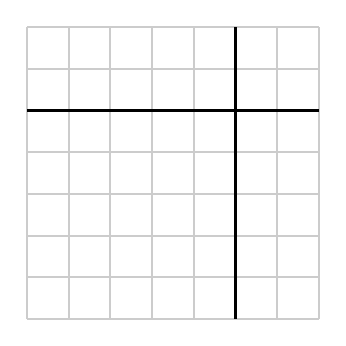
\includegraphics{figures/1_8_Act1.eps}
\caption{Axes for plotting $y = L(x)$ and $y = g(x)$.} \label{F:1.8.Act1}
\end{center}
\end{figure}
\end{activity}

\begin{smallhint}
\ba
	\item Follow the rule for $L$.
	\item Recall that the form of the local linearization is $L(x) = g(a) + g'(a)(x-a)$.
	\item Is the function $g$ increasing or decreasing at $a = -1$?
	\item Remember that $g(-1.03) \approx L(-1.03)$.
	\item What does the second derivative tell you about the shape of a curve?
	\item Use your work above.
\ea
\end{smallhint}

\begin{bighint}
\ba
	\item Follow the rule for $L$ and note that you can easily compute $L'(x)$.
	\item Recall that the form of the local linearization is $L(x) = g(a) + g'(a)(x-a)$.  What is the value of $a$ for the given function $L$?
	\item Observe that the value of $g'(-1)$ tells you whether the function $g$ increasing or decreasing at $a = -1$.
	\item Remember that $g(-1.03) \approx L(-1.03)$ and you know a rule for $L(x)$.
	\item What does a positive second derivative tell you about the shape of a curve at a point?
	\item Use your work above, and think about the value, slope, and concavity of $y = g(x)$ at $a = -1$.
\ea
\end{bighint}




\aftera